\chapter{Majority Rule Map}
\ifpdf
    \graphicspath{{Chapter3/Chapter3Figs/PNG/}{Chapter3/Chapter3Figs/PDF/}{Chapter3/Chapter3Figs/}}
\else
    \graphicspath{{Chapter3/Chapter3Figs/EPS/}{Chapter3/Chapter3Figs/}}
\fi

\section{Computing the Majority Rule Map $P_{maj}$}

\subsection{Construction}
The following example taken from \cite{key1} demonstrates the construction of a majority rule map.

\begin{figure}[h]
\begin{center}
\scalebox{0.50}{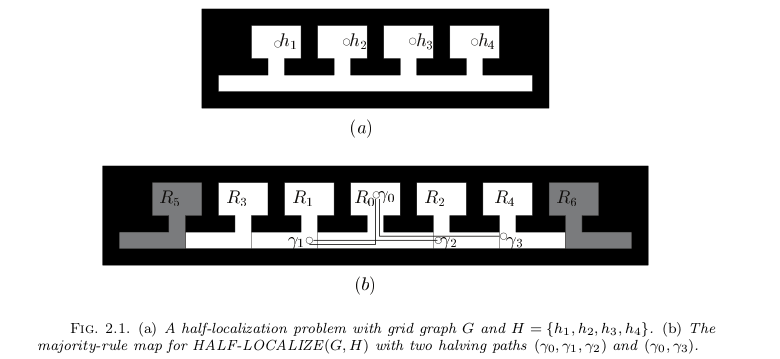
\includegraphics{Images/MajorityMapExample.png}}
\caption{\label{fig:Construction}Majority Rule Map Construction}
\end{center}
\end{figure}

${h_{1},h_{2},h_{3},h_{4}}$ form the set of hypotheses. Arbitrarily we choose $h_{1}$ as the origin. Next we translate all the 
remaining hypotheses to $h_{1}$ to obtain the overlay arrangement. The overlay arrangement contains the following faces
$R_{0},R_{1},R_{2},R_{3},R_{4},R_{5},R_{6}$. Recall from the definition of $Maj(\gamma)$



$  Maj(R_{0})  =  {h_{1}, h_{2}, h_{3}, h_{4}} $ , $  Maj(R_{1})  =  { h_{2}, h_{3}, h_{4}} $, $ Maj(R_{2})  =  {h_{1}, h_{2}, h_{3}} $,
$  Maj(R_{3})  =  {h_{3}, h_{4}} $ and $  Maj(R_{4})  =  {h_{1}, h_{2}} $



In the majority rule map the region $R_{5}$ and $R_{6}$ are blocked because less than half the hypothesis said that they were
 traversable. They have been shown in gray.

\begin{figure}[h]
\begin{center}
\scalebox{0.40}{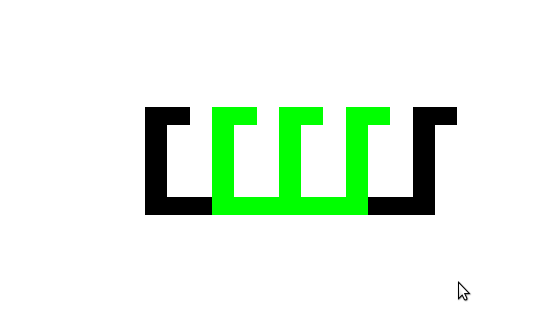
\includegraphics{Images/MajorityMapScenario1.png}}
\caption{\label{fig:Majority Rule Map}Majority Rule Map shown in green}
\end{center}
\end{figure}





\newpage
\subsection{Majority Rule Map Type}

The Majority Rule Map is represented as a class. The following code demonstrates the values stored along with a majority rule map and the 
functions applicable on it.




%%%%%%%%%%%%%%%%%%%%%%%%%%%%%%%%%%%%%%%%%%%%%%%%%%%%%%%%%%%%%%%
%  Java Sourcecode to TeX automatically converted code
%  Java2Html Converter 5.0 [2006-02-26]by Markus Gebhard  markus@jave.de
%     Further information: http://www.java2html.de
{
\noindent \ttfamily
\jttstylea \\
\jttstylea \\
\jttstylea \\
\jttstylea \\
\jttstylee class~\jttstylek Majoritymap~\jttstylei \{\\
\jttstylee public\jttstylek :\\
\jttstylea \\
\jttstylea ~~\jttstylek list\verb#<#Faces\verb#>#~listMmapFaces;\\
\jttstylea ~~\jttstylek Polygon~map;\\
\jttstylea ~~\jttstylej int~\jttstylek noOfHypothesis;\\
\jttstylea ~~\jttstylek Point~\verb#*#hypothesis;\\
\jttstylea ~~\jttstylek Point~center;\\
\jttstylea ~~\jttstylek list\verb#<#Polygon\verb#>#~listTanslatedPolygons;\\
\jttstylea ~~\jttstylek Arrangement~mmapArrangement;\\
\jttstylea \\
\jttstylea ~~\jttstylek PolygonUtil~pUtil;~\jttstyled //For~using~polygon~util~functions.\\
\jttstylea \\
\jttstylea ~~\jttstylek Majoritymap\jttstylei ()\jttstylek ;\\
\jttstylea ~~\jttstylek Majoritymap\jttstylei (\jttstylej int~\jttstylek n,~Point~H\jttstylei []\jttstylek ,Point~c,Polygon~P\jttstylei )\jttstylek ;\\
\jttstylea ~~\jttstylek Majoritymap\jttstylei (\jttstylej int~\jttstylek n,std::list\verb#<#Polygon\verb#>#~PolygonList\jttstylei )\jttstylek ;\\
\jttstylea \\
\jttstylea \\
\jttstylea ~~\jttstylej void~\jttstylek PrintMajorityMap\jttstylei ()\jttstylek ;\\
\jttstylea ~~\jttstylej void~\jttstylek GenerateMajorityMap\jttstylei ()\jttstylek ;\\
\jttstylea ~~\jttstylek Polygon~GetTranslatePolygon\jttstylei (\jttstylek Transformation\&~translate,~Polygon\&~polygon\jttstylei )\jttstylek ;\\
\jttstylea ~~\jttstylek Polygon~ConvertFaceToPolygon\jttstylei (\jttstylek Arrangement::Ccb\verb#_#halfedge\verb#_#const\verb#_#circulator~circ\jttstylei )\jttstylek ;\\
\jttstylea ~~\jttstylek bool~IsContainedIn\jttstylei (\jttstylek Polygon~outer,Polygon~inner\jttstylei )\jttstylek ;\\
\jttstylea ~~\jttstylek bool~CheckPartOfMajorityMap\jttstylei (\jttstylej int~\jttstylek agree,~\jttstylej int~\jttstylek noOfHypothesis\jttstylei )\jttstylek ;\\
\jttstylea \\
\jttstylea ~~\jttstylek list\verb#<#Polygon\verb#>#~findRegionContaningOrigin\jttstylei ()\jttstylek ;\\
\jttstylea ~~\jttstylek bool~areAdjacent\jttstylei (\jttstylek Polygon\&~poly1,~Polygon\&~poly2\jttstylei )\jttstylek ;\\
\jttstylea \\
\jttstylea ~~\jttstylek Polygon~OverlayContaningOrigin\jttstylei (\jttstylek Point~\&center\jttstylei )\jttstylek ;\\
\jttstylea \\
\jttstylea ~~\jttstylej void~\jttstylek GenerateOverlay\jttstylei (\jttstylek list\verb#<#Polygon\verb#>#~polygonList\jttstylei )\jttstylek ;\\
\jttstylea ~~\jttstylej void~\jttstylek partMajority\jttstylei ()\jttstylek ;\\
\jttstylea ~~\jttstylek virtual~\verb#~#Majoritymap\jttstylei ()\jttstylek ;\\
\jttstylei \}\jttstylek ;\\
\jttstylea \\
\jttstylea \\
\jttstylea \\
\jttstylea \jttstylea 
\\

}

Each majority rule map is basically a collection of faces. Faces is another type that encapsulates information about the opinion of 
each of the hypotheses about that face. Here is the Faces class.

%%%%%%%%%%%%%%%%%%%%%%%%%%%%%%%%%%%%%%%%%%%%%%%%%%%%%%%%%%%%%%%
%  Java Sourcecode to TeX automatically converted code
%  Java2Html Converter 5.0 [2006-02-26]by Markus Gebhard  markus@jave.de
%     Further information: http://www.java2html.de
{
\noindent \ttfamily
\jttstylea \\
\jttstylee class~\jttstylek Faces~\jttstylei \{\\
\jttstylee public\jttstylek :\\
\jttstylea ~~\jttstylek Polygon~face;\\
\jttstylea ~~\jttstylej int~\jttstylek noOfHypothesis;\\
\jttstylea ~~\jttstylek bool~\verb#*#containedIn;\\
\jttstylea ~~\jttstylek bool~partOfMajorityMap;\\
\jttstylea ~~\jttstylek Faces\jttstylei ()\jttstylek ;\\
\jttstylea ~~\jttstylek Faces\jttstylei (\jttstylej int~\jttstylek n,Polygon~p,~bool~\verb#*#A,bool~partMmap\jttstylei )\jttstylek ;\\
\jttstylea ~~\jttstylek Faces\jttstylei (\jttstylek Polygon~p\jttstylei )\jttstylek ;\\
\jttstylea ~~\jttstylej void~\jttstylek PrintDescription\jttstylei ()\jttstylek ;\\
\jttstylea ~~\jttstylek virtual~\verb#~#Faces\jttstylei ()\jttstylek ;\\
\jttstylei \}\jttstylek ;\\

}

Each Face has a bool flag partOfMajorityMap, which is true if this face is a part of the majority map i.e. atleast half of the 
hypotheses say that this face is traversable and false otherwise. It also has an bool array to specifically store the opinion of
 each of the hypothesis about this face.

\newpage
\subsection {CGAL's Arrangement class to generate Overlay}



%Java2TeX style definitions
%You can modify them to fit your needs

%%%%%%%%%%%%%%%%%%%%%%%%%%%%%%%%%%%%%%%%%%%%%%%%%%%%%%%%%%%%%%%
%  Java Sourcecode to TeX automatically converted code
%  Java2Html Converter 5.0 [2006-02-26]by Markus Gebhard  markus@jave.de
%     Further information: http://www.java2html.de
{
\noindent \ttfamily
\jttstylea \\
\jttstylea \\
\jttstylea \\
\jttstylej void~\jttstylek Majoritymap::GenerateOverlay\jttstylei (\jttstylek list\verb#<#Polygon\verb#>#~polygonList\jttstylei )\\
\jttstylei \{\\
\jttstylea \\
\jttstylea ~~\jttstylek list\verb#<#Polygon\verb#>#::iterator~pi;\\
\jttstylea \\
\jttstylea ~~\jttstylee for\jttstylei (\jttstylek pi=polygonList.begin\jttstylei ()\jttstylek ;pi!=polygonList.end\jttstylei ()\jttstylek ;++pi\jttstylei )\\
\jttstylea ~~\jttstylei \{\\
\jttstylea ~~~~\jttstylee for~\jttstylei (\jttstylek EdgeIterator~ei~=~pi-\verb#>#edges\verb#_#begin\jttstylei ()\jttstylek ;~ei~!=~pi-\verb#>#edges\verb#_#end\jttstylei ()\jttstylek ;~++ei\jttstylei )\\
\jttstylea ~~~~\jttstylei \{\\
\jttstylea ~~~~~~\jttstylek Point~s=ei-\verb#>#start\jttstylei ()\jttstylek ;\\
\jttstylea ~~~~~~\jttstylek Point~d=ei-\verb#>#end\jttstylei ()\jttstylek ;\\
\jttstylea ~~~~~~\jttstylek Point\verb#_#2~source\jttstylei (\jttstylek s.cartesian\jttstylei (\jttstyleh 0\jttstylei )\jttstylek ,s.cartesian\jttstylei (\jttstyleh 1\jttstylei ))\jttstylek ;\\
\jttstylea ~~~~~~\jttstylek Point\verb#_#2~destination\jttstylei (\jttstylek d.cartesian\jttstylei (\jttstyleh 0\jttstylei )\jttstylek ,d.cartesian\jttstylei (\jttstyleh 1\jttstylei ))\jttstylek ;\\
\jttstylea ~~~~~~\jttstylek Segment\verb#_#2~seg\jttstylei (\jttstylek source,~destination\jttstylei )\jttstylek ;\\
\jttstylea ~~~~~~\jttstylek CGAL::insert~\jttstylei (\jttstylek mmapArrangement,seg\jttstylei )\jttstylek ;\\
\jttstylea ~~~~\jttstylei \}\\
\jttstylea ~~\jttstylei \}\\
\jttstylea \\
\jttstylea \\
\jttstylea ~~\jttstylek Arrangement::Face\verb#_#const\verb#_#iterator~fit;\\
\jttstylea \\
\jttstylea ~~\jttstylee for~\jttstylei (\jttstylek fit~=~mmapArrangement.faces\verb#_#begin\jttstylei ()\jttstylek ;~fit~!=~mmapArrangement.faces\verb#_#end\jttstylei ()\jttstylek ;~++fit\jttstylei )\\
\jttstylea ~~\jttstylei \{\\
\jttstylea ~~~~\jttstylee if~\jttstylei (\jttstylek !fit-\verb#>#is\verb#_#unbounded\jttstylei ())\\
\jttstylea ~~~~\jttstylei \{\\
\jttstylea ~~~~~~\jttstylek Polygon~p=ConvertFaceToPolygon\jttstylei (\jttstylek fit-\verb#>#outer\verb#_#ccb\jttstylei ())\jttstylek ;\\
\jttstylea ~~~~~~\jttstylek Faces~f\jttstylei (\jttstylek p\jttstylei )\jttstylek ;\\
\jttstylea ~~~~~~\jttstyled //constructing~the~overlay~Arrangement~by~adding~the~faces~as~polygons.\\
\jttstylea ~~~~~~\jttstylek listMmapFaces.push\verb#_#back\jttstylei (\jttstylek f\jttstylei )\jttstylek ;\\
\jttstylea ~~~~\jttstylei \}\\
\jttstylea \\
\jttstylea ~~\jttstylei \}\\
\jttstylei \}\\
\jttstylea \\
\jttstylea \jttstylea 
\\

}
First we insert all edges in the region using CGAL::insert (mmapArrangement,seg). The Arrangement class which is inbuilt in CGAL 
automatically generates all faces that can be formed by the intersection of the edges.





\subsection{Algorithm}
\begin{enumerate}
\item
The overlay arrangement can be easily constructed using CGAL's inbuilt Arrangement class. Obtain the translates of the polygon by 
choosing one hypothesis as the origin and shifting other hypothesis to it.
\item
Insert all these translates in CGAL's inbuilt arrangement to obtain all the faces in the overlay arrangement.
\item
Faces which belong to atleast half the hypothesis are marked as part of the majority rule map.
\end{enumerate}


\subsection{Examples}


\begin{figure}[h]
\begin{center}
\scalebox{0.50}{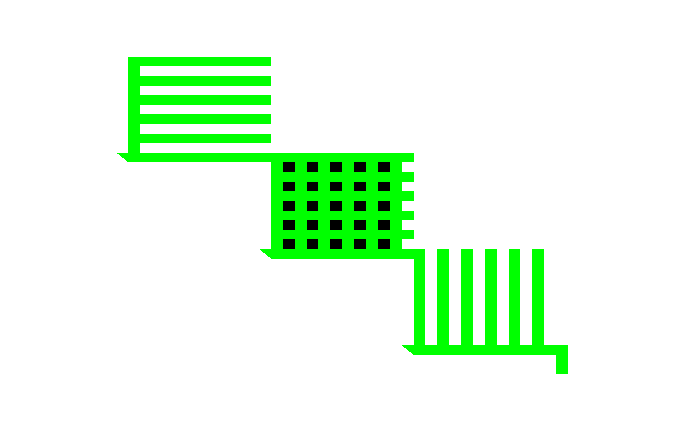
\includegraphics{Images/MajorityMapScenario4.png}}
\caption{\label{fig:Majority Rule Map}Majority Rule Map}
\end{center}
\end{figure}


% ------------------------------------------------------------------------


%%% Local Variables: 
%%% mode: latex
%%% TeX-master: "../thesis"
%%% End: 
